
\section{Requirements and System Model}\label{sec:requirements}
Big data is highly dependent on cloud-edge computing, which makes extensive use of multitenancy.
Multitenancy permits sharing one instance of infrastructures, platforms or applications by multiple tenants to optimize costs.
This leads to common scenarios where a service provider offers subscription-based analytics capabilities in the cloud,
or a single data lake is accessed by multiple customers.
Thus, it is a common situation to have a big data pipeline where data and services belong to various organizations,
posing a serious risk of potential privacy and security violation.
The fundamental concept underlying our methodology is to enhance the prevailing paradigm for big data pipelines through the creation of a Data Governance framework tailored to contemporary data-driven pipelines.
The primary objective of this framework is to facilitate the assembly of data processing services, with a central focus on the selection of these services to optimize data quality, all while upholding privacy standards.
In the following of this section,
we present our system model (Section \ref{sec:systemmodel}),
and our reference scenario (Section \ref{sec:reference}).

\subsection{System Model}\label{sec:systemmodel}

Our guiding principle is to balance two critical imperatives: data quality and data privacy.
In today's data landscape, the coexistence of data quality and data privacy is critical.
The increase in data production has led to a split in scientific research priorities. This has resulted in two main areas of focus.
First, researchers are exploring methods to optimize valuable data. Here, ensuring data quality is vital, and requires accuracy, reliability, and suitability for analytical purposes.
Second, there is a need to prioritize data privacy and security. This involves safeguarding confidential information and complying with strict privacy regulations.
These two directions are happening at the same time, but there are not many solutions that find a good balance between them.
Our approach seeks to harmonize these objectives by establishing a framework that balances privacy and data quality.xw

Our system model is composed by the following parties:

It includes the following parties:
\begin{description}
  \item[User] the entity that wants to perform some analytics on the data
  \item[Pipeline] a sequence of connected services that process and move data from one point to another in a structured and automated manner.
  \item[Service] a software that performs a specific task, a service can be tagged with some policies %, a service is characterized by two function: the service function and the policy function.
  \item[Data Governance Policy] a structured set of guidelines, rules, and procedures that define how the service must safeguards its data to maintain confidentiality
  \item[Template] Empty pipeline that acts as a skeleton, containing necessary but empty steps, to be filled with specific services ( Figure \ref{fig:service_composition_template}). Each step can be annotated with a policy.

\end{description}


In our context, a \user aims to execute a data pipeline to perform analysis or transformation procedures on some data.
The input data are considered already cleaned, this means having undergone a preparatory phase that has addressed issues such as missing values,
outliers, and formatting discrepancies, ensuring that the data are in an optimal state for subsequent analysis.
% Policies governing the data are established, which can originate from the \user, third-party entities, or regulatory frameworks.
% For instance, a policy may restrict the execution of processing operations to a specific geographic region.
The \user is presented with a list of empty pipeline templates.
When the template is selected, users are presented with lists of candidate services that are equivalent in functionality and comply with the policies specified in the template.
Services are ranked based on their ability to retain the maximum amount of information while maintaining an equivalent level of privacy.
Priority is given to the service that maximizes data quality while maintaining the same level of privacy.
Our investigation presumes that upholding a larger quantity of data is linked to better data quality.
This evaluation process aids in identifying the most suitable service for a particular step in the pipeline.
Upon selecting the most suitable service for each step, the pipeline instantiation is considered complete and ready for execution.
It is important to emphasize that our goal is not to formulate novel service composition algorithms, but rather to establish a data governance framework.

\subsection{Reference Scenario}\label{sec:reference}
Our reference scenario is a service-based environment where services are composed according to a pipeline template.
The case study is based on an analysis of a dataset consisting of individuals detained in Department of Correction facilities in the state of Connecticut while awaiting trial.
The dataset\footnote{https://data.ct.gov/Public-Safety/Accused-Pre-Trial-Inmates-in-Correctional-Faciliti/b674-jy6w}, exhibits a straightforward row-and-column structure.
Each row represents an inmate, and the columns include the following attributes: date of download, a unique identifier, last entry date, "race," gender, age of the individual, the bound value, offense, entry facility, and detainer.
To serve the objectives of our study, we have extended this dataset by introducing randomly generated first and last names.
We envision the establishment of a service pipeline designed as follows:
The end user, a member of the Connecticut Department of Correction (DOC),
seeks to perform an analysis on the dataset to compare admission trends in Connecticut prisons with those in other states.
The user's preferences align with a predefined template that orchestrates the following sequence of operations:
i) Anonymization of the dataset.
ii) Expansion of the dataset, integrating data from the states of New York and New Hampshire.
iii) Transformation of the dataset to derive state-specific data aggregations, including statistical measures like averages, medians, and clustering-based statistics.
iv) Storage of the resultant data in reference states. Specifically, one copy remains in Connecticut (where sensitive information in the source dataset is not protected), while two additional copies are distributed to New York and New Hampshire (with sensitive information from the source dataset being safeguarded).

It should be noted that the template requires the execution of the entire service within a single country.
In cases where the data needs to be transmitted beyond the boundaries of Connecticut, data protection measures are implemented.
A visual representation of the flow is presented in Figure \ref{fig:service_composition_example}.

\begin{figure}
  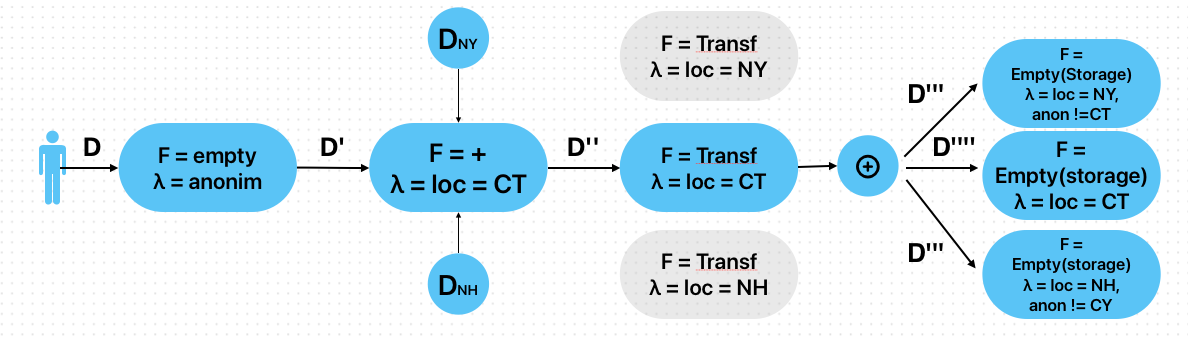
\includegraphics[width=0.98\columnwidth]{service_composition_example}
  \caption{Service composition example.}\label{fig:service_composition_example}

\end{figure}



\section{Service}
\subsection{Service Definition}
Within the framework, a service is defined as an entity that receives input data, processes it by applying a transformation function, and produces an output result.
Each service essentially consists of the  service transformation function (\F{}).
The transformation function can be of 4 main types:
\begin{enumerate*}[label=\roman*)]
  \item \F{Empty} The function applies no transformation or processing on the data.
  \item \F{additive} The function expands the amount of data received, for example, by integrating it with data from other sources.
  \item \F{transformation} The function transforms some records in the dataset without altering the domain.
  \item \F{domain change }  The function changes the domain of the data by applying e.g. PCA or K-means (will not be considered in the current work).
\end{enumerate*}


Each service can be chained with other services to form a service flow.
A service flow is defined as a graph. G(\V, \E, \F{}) where \V is a set of vertices, \E is a set of edges, and F is a set of functions.
Each vertex in V represents a service, and each edge in E represents a data flow between two services.
Each function in F represents a transformation function that is applied to the data.

% \begin{definition}[Big Data Analytics Pipeline] \label{def:pipeline}
%   A Big Data Analytics pipeline \G(\V,\E) is a direct acyclic graph having a root \vi{r}$\in$\V, a vertex \vi{i}$\in$\V$_I$$\subseteq$\V\ for each job \job{i} invocation, two additional vertices \vi{c},\vi{m}$\in$\V$_{\otimes}$$\subset$\V\ for each alternative ($\otimes$) structure modeling the alternative execution (\emph{choice}) of operations and the retrieval (\emph{merge}) of the results,
%     respectively, and two additional vertices \vi{f},\vi{j}$\in$\V$_{\oplus}$$\subset$\V\ for each parallel ($\oplus$) structure modeling the contemporary execution (\emph{fork}) of operations and the integration (\emph{join}) of their results, respectively.
% \end{definition}

% We note that each vertex \vi{i} model a job \job{i} provided by an organization \org{i}.
% We also note that an analytics pipeline can be deployed following a centralized or a decentralized approach as discussed in detail in Section \ref{sec:architecture}.

\begin{figure}[!t]
  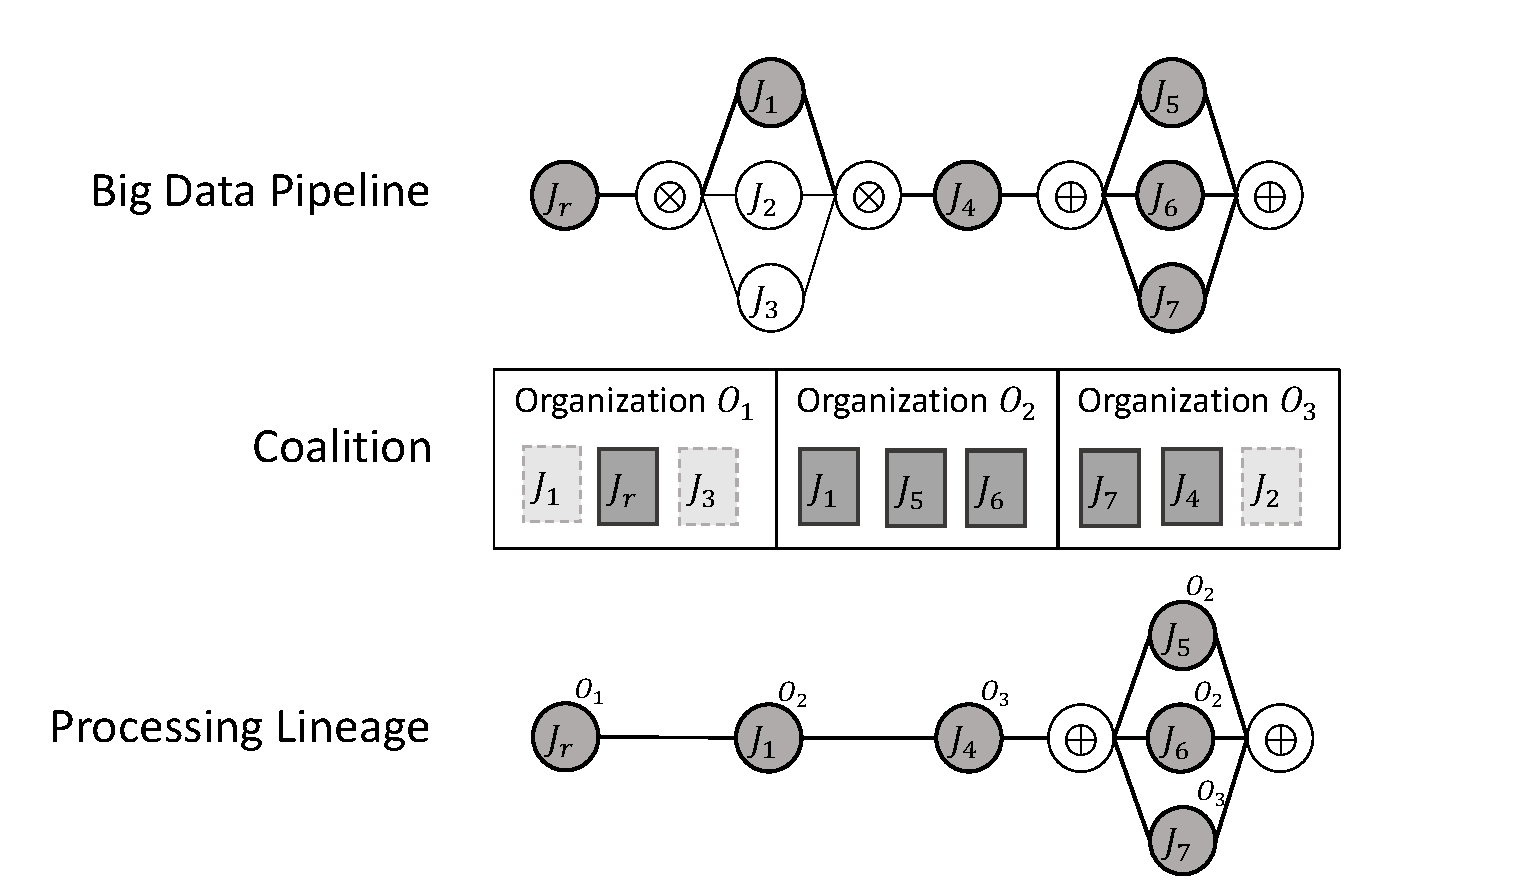
\includegraphics[width=0.98\columnwidth]{generaleFig1.pdf}
  \caption{Big Data Analytics pipeline graphs with a coalition of organization for a given processing lineage.}\label{fig:BDpipeline}
\end{figure}

Figure~\ref{fig:BDpipeline} shows an overview of our system model.

%Solid arrows present the typical batch or analytics model generation flows. Dashed arrows present typical streaming or prediction flows. \CH{togliere dalla figura la linea che separa le due procedure e le scritte ingestion procedure e analytics procedure?}
%The coalition creation is driven by missions including emergency and disaster management, humanitarian operations, or simply interdependent organizations.
%\CH{Qui ho introdotto solo il termine coalition, va spiegato anche il termine federation?}





\section{Service Template}
\subsection{Definition}
The main point of our investigation is a service-based environment where services are combined strategically with policies that cater to the specific needs of the user.
Our focus is on service composition, which involves three main actors and operates at a higher level of abstraction.
\begin{enumerate}
  % \item The \User:
  %       The stakeholder within the service-based environment,
  %       the \user assumes the role of the entity initiating the request for a particular service.
  %       By choosing a template, the \user initiate the subsequent stages of the composition process.
  \item The Service Template:
        At the crux of effective service composition lies the pivotal role played by the service template.
        Functioning as a high-level composition of services labeled with predefined policies,
        the service template serves as a structured blueprint facilitating the decision-making process for the  \user.
        \begin{definition}[Service Template] \label{def:pipeline}
          A Service Template \T(\V,\E,$\iChartFunction{}$), is a direct acyclic graph having a root \vi{r}$\in$\V, a vertex \vi{i}$\in$\V\ for each service $s_i$,
          two additional vertices \vi{c},\vi{m}$\in$\V$_{\timesOperator}$$\subset$\V\ for each alternative ($\timesOperator$) structure modeling the alternative execution (\emph{choice}) of operations and the retrieval (\emph{merge}) of the results,
                respectively, and two additional vertices \vi{f},\vi{j}$\in$\V$_{\plusOperator}$$\subset$\V\ for each parallel ($\plusOperator$) structure modeling the contemporary execution (\emph{fork}) of operations and the integration (\emph{join}) of their results, respectively. $\iChartFunction{}$ is an annotation function, assigning to each vertex \vi{i}$\in$\V\ a set of policies \Pset{i}.
        \end{definition}
        % We note that $\{$\vi{r}$\}$ $\cup S_\timesOperator\cup S_\plusOperator=S$\\
  \item The Service Provider:
        Central to the execution of service composition is the service provider,
        serving as the responsible entity for delivering the requested service.
        Tasked with adhering to the prescribed service template, the service provider execute the service requested by the \user.
\end{enumerate}

% More detail about the structure modeling the alternative and parallel follows :

% \textbf{Sequence} ($\plusOperator$). It composes two service, $wsi$ and $wsj$, in a sequence. $wsi\plusOperator wsj$ mimics a composition where $wsj$ is executed after $wsi$.

% \textbf{Alternative} ($\timesOperator$). It composes two service, $wsi$ and $wsj$, in an alternative. $wsi\timesOperator wsj$ mimics a composition where either $wsi$ or $wsj$ is executed.

% \textbf{Parallel} ($\plusOperator$). It composes two service, $wsi$ and $wsj$, in parallel. $wsi\plusOperator wsj$ mimics a composition where both $wsi$ and $wsj$ are executed simultaneously.
\begin{figure}[h!]
  \centering
  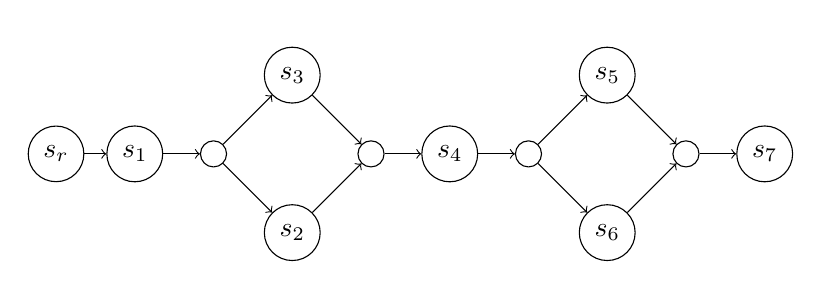
\begin{tikzpicture}
    % Nodes
    \node[draw, circle] (node1) at (0,0) {$s_r$};
    \node[draw, circle] (node2) at (1,0) {$s_1$};
    \node[draw, circle] (node3) at (2,0) {$\timesOperator$};
    \node[draw, circle] (node4) at (3,-1) {$s_2$};
    \node[draw, circle] (node5) at (3,1) {$s_3$};
    \node[draw, circle] (node6) at (4,0) {$\timesOperator$};
    \node[draw, circle] (node65) at (5,0) {$s_4$};
    \node[draw, circle] (node7) at (6,0) {$\plusOperator$};
    \node[draw, circle] (node8) at (7,1) {$s_5$};
    \node[draw, circle] (node9) at (7,-1) {$s_6$};
    \node[draw, circle] (node10) at (8,0) {$\plusOperator$};
    \node[draw, circle] (node11) at (9,0) {$s_7$};
    % Text on top
    \node[above] at (node1.north)  {$\tChartFunction$};
    \node[above] at (node2.north)  {$\tChartFunction$};
    \node[above] at (node3.north)  {                 };
    \node[above] at (node4.north)  {$\tChartFunction$};
    \node[above] at (node5.north)  {$\tChartFunction$};
    \node[above] at (node65.north) {$\tChartFunction$};
    \node[above] at (node8.north)  {$\tChartFunction$};
    \node[above] at (node9.north)  {$\tChartFunction$};
    \node[above] at (node11.north) {$\tChartFunction$};
    % Connection
    \draw[->] (node1) -- (node2);
    \draw[->] (node2) -- (node3);
    \draw[->] (node3) -- (node4);
    \draw[->] (node3) -- (node5);
    \draw[->] (node5) -- (node6);
    \draw[->] (node4) -- (node6);
    \draw[->] (node6) -- (node65);
    \draw[->] (node65) -- (node7);
    \draw[->] (node7) -- (node8);
    \draw[->] (node7) -- (node9);
    \draw[->] (node8) -- (node10);
    \draw[->] (node9) -- (node10);
    \draw[->] (node10) -- (node11);
  \end{tikzpicture}
  \caption{Service composition template}
  \label{fig:service_composition_template}
\end{figure}

\subsection{Policy}
% \subsubsection{Annotations}
% \subsubsection{Transformation}

\subsubsection{Policy Decision/Policy Matching}
\subsubsection{Policy Enforcement}
\subsubsection{Policy Evaluation}